\subsection{Méthode de modélisation}
      \paragraph{}
      Afin de modéliser les fonctionnalités de notre solution, nous avons choisi le langage UML \textit{Unified Modeling Language} \cite{I}. Issu d’un large consensus, le langage UML garantit la stabilité et la performance d’un projet grâce à son caractère formel et industrialisé. Aussi facilite-t-il la compréhension du système par l’usage de représentations graphiques appelées diagrammes. Ces derniers nous ont permis de modéliser notre solution en utilisant les diagrammes de cas d’utilisation et de séquence.\\ \\
\subsection{Diagramme de cas d'utilisation}
    \paragraph{}
	  Le diagramme de cas d'utilisation représente la structure des grandes fonctionnalités nécessaires aux utilisateurs du système. C'est le premier diagramme du modèle UML, celui où s'assure la relation entre l'utilisateur et les objets que le système met en œuvre. 

	  \begin{figure}[H]
		     \begin{center}
			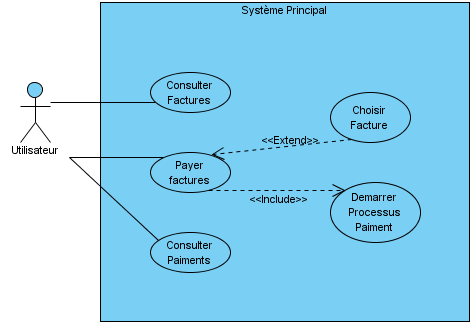
\includegraphics[scale=0.5]{images/uc.png}
		     \end{center}
		     \caption{Diagramme de cas d'utilisation}
		     \label{Diagramme de cas d'utilisation}
	  \end{figure}
	  
	  Pour une premi\`ere utilisation, il est n\'ecessaire de cr\'eer un compte. Les informations \`a fournir sont: un nom, un email, un num\'ero de t\'el\'ephone, la r\'ef\'erence abonn\'ee et le mot de passe pour la protection du compte. Ces informations sont obligatoires. Un mail d'activation est envoy\'e et l'utilisateur apr\`es activation de son compte peut se connecter \`a l'application. Une authentification est nécessaire afin d'avoir acc\`es aux cas d'utilisations de notre diagramme (ou aux fonctionnalités de l'application). Sur notre diagramme de cas d'utilisation, nous pouvons identifier un client et un administrateur. Le client peut consulter et payer ses factures, et il peut aussi voir ses paiements. L'administrateur quant \`a lui g\`ere les comptes abonn\'es et \`a acc\`es \`a certaines informations comme le nombre de factures d\'ej\`a vendues au cours de la journ\'ee et le montant total.
	  
\subsection{Diagramme de séquence}
 \paragraph{}
	  Le diagramme de séquence représente la succession chronologique des opérations réalisées par un acteur. Ce mode de représentation effectue la description du fonctionnement dynamique du système. En d'autres termes, il indique les objets que l'acteur va manipuler et les opérations qui font passer d'un objet à l'autre.
	  \begin{figure}[H]
		     \begin{center}
			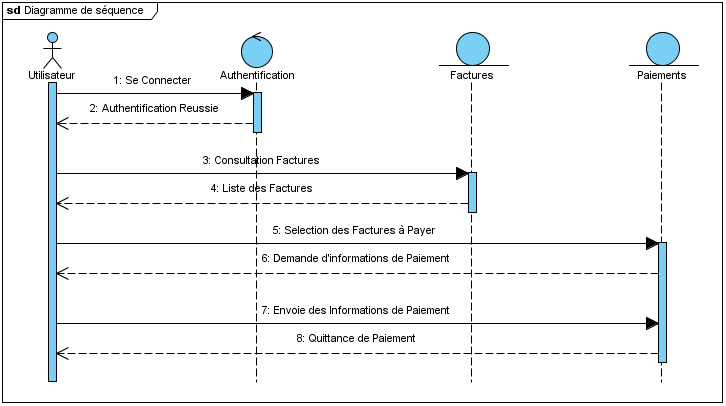
\includegraphics[scale=0.6]{images/sd.png}
		     \end{center}
		     \caption{Diagramme de séquence}
		     \label{Diagramme de cas d'utilisation}
	  \end{figure}
	  \paragraph{}
	  Après que l'utilisateur ait entré ses informations, identifiants pour se connecter, il a acc\`es aux factures. L\`a il peut ajouter les factures impay\'ees \`a la liste des factures \`a payer (m\^eme concept que le panier d'un site d'e-commerce). Il pourra donc proc\'eder au paiement de ses factures via le mode de paiement qui lui convient. Une quittance lui est g\'en\'er\'ee et est ajout\'ee \`a son historique de paiements.